\documentclass[t,% Place text of slides at the (vertical) top of the slides
brazilian,% Brazilian Portuguese, FTW!
11pt,% Standard font size
aspectratio=169,% Aspect ratio 16:9 (widescreen)
table% xcolor option
]{beamer}

\usetheme{Boadilla}
\setbeamertemplate{navigation symbols}{}
\setbeamertemplate{frametitle continuation}{}
\setbeamertemplate{page number in head/foot}[framenumber]
\setbeamertemplate{enumerate items}[default]
\setbeamertemplate{itemize items}[circle]
\setbeamercovered{transparent}
\setbeamerfont{frametitle}{size=\normalsize}

\usepackage{babel}
\usepackage[utf8]{inputenc}
\usepackage[T1]{fontenc}
\usepackage{lmodern}

\usepackage{graphicx}
\usepackage{tikz}

\usepackage{amssymb,amsfonts,amsmath}
\usepackage{mathtools}

\usepackage{siunitx}

\usetikzlibrary{calc}
\usetikzlibrary{intersections}
\usetikzlibrary{matrix,positioning}

\setkeys{Gin}{keepaspectratio}
\sisetup{locale = FR}

\DeclareMathOperator{\sen}{sen}
\DeclareMathOperator{\arcsen}{arc sen}
\renewcommand{\vec}[1]{\overrightarrow{#1}}

\usepackage{tcolorbox}
\tcbset{boxrule=0pt, top=0pt, bottom=0pt}

\usepackage{pgfplots}
\pgfplotsset{compat=newest}

\usepgfplotslibrary{fillbetween}

\usepackage{pgfcalendar}
\usepackage{xstring}
\usepackage{array}
\newcolumntype{P}[1]{>{\centering\arraybackslash}p{#1}}

\newcommand{\feriados}{07/04/2023,21/04/2023,25/04/2023,01/05/2023,08/06/2023,29/06/2023}
\newcommand{\inicio}{2023-03-20}

\newcommand{\dma}[1]{
    \newcount\mycount
    \pgfcalendardatetojulian{\inicio+#1}{\mycount}
    \pgfcalendarjuliantodate{\mycount}{\myyear}{\mymonth}{\myday}
    \IfSubStr{,\feriados,}{,\myday/\mymonth/\myyear,}{\cellcolor{red!20}}{}
    \myday/\mymonth
}

\usepackage{qrcode}
%--------------------------------------------------

\def\Disciplina{Métodos Numéricos}
\def\Professor{Rodrigo de Farias Gomes}
\def\Periodo{Período 2022.2}

\title{\Disciplina}
\author{\Professor}
\date{\Periodo}

% Macros for ``successive divisions'' 
%
\def\Division#1#2#3{ % Dividend, divisor, remainder
 \matrix (D) [matrix of nodes,
              below=0pt of D-1-2.south east,
              row sep=1pt, column sep=1pt,
              every node/.append style={minimum width=12mm}] {
   #1 \pgfmatrixnextcell #2 \\
   |[marcar] (R#1)| #3      \\
 };
 \draw[shorten >=2pt, shorten <=2pt]
   (D-1-2.north west) |- (D-1-2.south east);
}
\def\FinDivision#1{
\node[marcar, below=2pt of D-1-2.south] (C)(C)  {#1};
}
\tikzset{marcar/.style={circle,draw,inner sep=2pt,minimum width=0pt,
fill=yellow!10}}
%
\usepackage{listings}
\lstset{
    frame=single, 
    basicstyle=\ttfamily, 
    keywordstyle=\color{blue!75},
    showstringspaces=false,
    commentstyle=\color{green!75!black}
}
\usepackage{inconsolata}

\begin{document}

\section{Apresentação}

\begin{frame} % Capa
    \titlepage
\end{frame}

\begin{frame}{Apresentação}
    \begin{itemize}
        \item Professor {\fontfamily{augie}\selectfont Rodrigo de Farias Gomes}
        \item Telefone (somente mensagens): (92) 9 9405-1724
        \item E-mail: shpnft@gmail.com

    \end{itemize}

    \centering

    \vspace{2cm}
    \begin{tabular}{cccccc}
        R & G & O & M & E & S \\ \\
        \(\color{red} \left.\phantom{{\scriptstyle +1}\frac{1}{2}}\right\downarrow {\scriptstyle +1}~~\) &
        \(\color{red} \left.\phantom{{\scriptstyle +1}\frac{1}{2}}\right\downarrow {\scriptstyle +1}~~\) &
        \(\color{red} \left.\phantom{{\scriptstyle +1}\frac{1}{2}}\right\downarrow {\scriptstyle +1}~~\) &
        \(\color{red} \left.\phantom{{\scriptstyle +1}\frac{1}{2}}\right\downarrow {\scriptstyle +1}~~\) &
        \(\color{red} \left.\phantom{{\scriptstyle +1}\frac{1}{2}}\right\downarrow {\scriptstyle +1}~~\) &
        \(\color{red} \left.\phantom{{\scriptstyle +1}\frac{1}{2}}\right\downarrow {\scriptstyle +1}~~\) \\ \\
        S & H & P & N & F & T
    \end{tabular}
\end{frame}

\begin{frame}{Calendário}
    \centering
    \small{
        \begin{tabular}{cP{2cm}P{2cm}P{2cm}P{2cm}P{2cm}}
            \rowcolor{black!10} & Segunda & Terça & Quarta & Quinta & Sexta \\
            01 & \dma{0} & \dma{1} & \dma{2} & \dma{3} & \dma{4} \\
            02 & \dma{7} & \dma{8} & \dma{9} & \dma{10} & \dma{11} \\
            03 & \dma{14} & \dma{15} & \dma{16} & \dma{17} & \dma{18} \\
            04 & \dma{21} & \dma{22} & \dma{23} & \dma{24} & \dma{25} \\
            05 & \dma{28} & \dma{29} & \dma{30} & \dma{31} & \dma{32} \\
            06 & \dma{35} & \dma{36} & \dma{37} & \dma{38} & \dma{39} \\
            07 & \dma{42} & \dma{43} & \dma{44} & \dma{45} & \dma{46} \\
            08 & \dma{49} & \dma{50} & \dma{51} & \dma{52} & \dma{53} \\
            09 & \dma{56} & \dma{57} & \dma{58} & \dma{59} & \dma{60} \\
            10 & \dma{63} & \dma{64} & \dma{65} & \dma{66} & \dma{67} \\
            11 & \dma{70} & \dma{71} & \dma{72} & \dma{73} & \dma{74} \\
            12 & \dma{77} & \dma{78} & \dma{79} & \dma{80} & \dma{81} \\
            13 & \dma{84} & \dma{85} & \dma{86} & \dma{87} & \dma{88} \\
            14 & \dma{91} & \dma{92} & \dma{93} & \dma{94} & \dma{95} \\
            15 & \dma{98} & \dma{99} & \dma{100} & \dma{101} & \dma{102} \\
            % 16 & \dma{103} & \dma{104} & \dma{105} & \dma{106} & \dma{107} \\
            % 17 & \dma{108} & \dma{109} & \dma{110} & \dma{111} & \dma{112} \\
        \end{tabular}
    }
\end{frame}

\begin{frame}{Meus horários em 20/03/2023...}
    \small{
        \begin{center}
            \begin{tabular}{ccccc}
                \rowcolor{black!10} Segunda & Terça & Quarta & Quinta & Sexta \\ \hline
                \rowcolor{red!25} &&&& \\ \hline
                \rowcolor{red!25} Métodos Num... & Trigonometria & Métodos Num... & Trigonometria & \\ \hline
                \rowcolor{green!25} & & Termodinâmica & & Termodinâmica \\ \hline
                \rowcolor{green!25} & Óptica e Eletro... & & Óptica e Eletro... & \\ \hline
                \rowcolor{blue!25} &&&& \\ \hline
                \rowcolor{blue!25} &&&& \\ \hline
            \end{tabular}
        \end{center}

        \vspace{1cm}
        Legenda:
        \begin{itemize}
            \item[\textcolor{red!25}{\rule{1em}{1em}}] Manhã (8:00 -- 10:00 e 10:00 -- 12:00)
            \item[\textcolor{green!25}{\rule{1em}{1em}}] Tarde (14:00 -- 16:00 e 16:00 -- 18:00)
            \item[\textcolor{blue!25}{\rule{1em}{1em}}] Noite (18:00 -- 20:00 e 20:00 -- 22:00)
        \end{itemize}
    }
\end{frame}

\begin{frame}{Ementa de \Disciplina}
    \begin{itemize}
        \item Erros e Sistemas de Numeração
        \item Solução de equações algébricas e transcendentais
        \item Solução de equações polinomiais
        \item Sistemas de equações lineares e não lineares
        \item Interpolação
        \item Ajustamento de curvas
        \item Integração numérica
        \item Solução numérica de equações diferenciais ordinárias e
            sistemas de equações diferenciais
    \end{itemize}
\end{frame}

\begin{frame}{Avaliação}
    \begin{itemize}
        \item A avaliação será na forma de 3 notas: \(N_1\), \(N_2\) e \(N_3\)
        \item A média dos exercícios escolares (\(MEE\)) será dada por
            \[
                MEE=\frac{N_1+N_2+N_3}{3}
            \]
        \item Se \(MEE \geq 8,0\), então a média final (\(MF\)) será igual à \(MEE\)
        \item Se \(MEE < 8,0\), então
            \[
                MF=\frac{2\times MEE+PF}{3}
            \]
            onde PF é a nota da \textbf{prova final}
        \item Se \(MF \geq 5,0\) e a frequência em sala for maior que 75\%, o aluno está aprovado
        \item Haverá 30 aulas de \SI{2}{horas}, de forma que \textbf{o número máximo de faltas é 8}
        % \item Google Sala de Aula:

        %     \centering
        %     https://classroom.google.com/c/NTQzNDU2NTQzODky?cjc=\textcolor{red}{i7z6ybp}
    \end{itemize}
\end{frame}

\begin{frame}{Google Sala de Aula}
    \centering
    \qrcode[height=0.8\textheight]{https://classroom.google.com/c/NTQzNDU2NTQzODky?cjc=i7z6ybp}
    \large{https://classroom.google.com/c/NTQzNDU2NTQzODky?cjc=\textcolor{red}{i7z6ybp}}
\end{frame}

\begin{frame}{Livro texto}
    \centering
    \includegraphics[height=0.8\textheight]{images/livro_burden.jpg}
    \includegraphics[height=0.8\textheight]{images/ruggiero.png}
\end{frame}

\begin{frame}{Solução analítica}
    \textbf{Soluções analíticas} são baseadas em fórmulas matemáticas em que
    são definidas variáveis de entrada para o cálculo de uma ou mais variáveis
    de saída. Por exemplo, a área de um segmento circular com raio \SI{2.0}{m}
    e profundidade \SI{1.0}{m}

    \begin{center}
        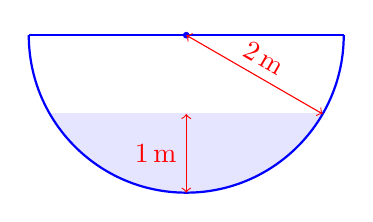
\begin{tikzpicture}[scale=1]
            \begin{scope}
                \clip (-2,-2) -| (2,-1) -| (-2,-2);
                \filldraw [blue!10] (-2,0) arc (180:360:2);
            \end{scope}
            \draw [thick,blue] (-2,0) arc (180:360:2);
            \draw [thick,blue] (-2,0) -- (2,0);
            \filldraw [blue] (0,0) circle (1pt);

            \draw [red, <->] (0,0) -- node [midway,sloped, above] {\SI{2}{m}} +(-30:2);
            \draw [red, <->] (0,-1) -- node [midway,left] {\SI{1}{m}} (0,-2);
        \end{tikzpicture}
    \end{center}
    é dada pela fórmula
    \[
        A=r^2 \arccos{\left(\frac{r-h}{r}\right)}-(r-h)\sqrt{r^2-(r-h)^2} 
        \approx \SI{2.4567}{m^2}
    \]
\end{frame}

\begin{frame}{Métodos numéricos}
    \textbf{Métodos numéricos} são fórmulas ou algoritmos usados para se obter
    \textbf{soluções aproximadas} para um problema matemático que,
    frequentemente, não tem solução analítica. Por exemplo, qual a profundidade
    de um segmento circular com raio \SI{2.0}{m} e área \(\SI{3.0}{m^2}\)?

    \begin{center}
        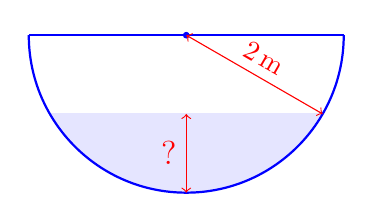
\begin{tikzpicture}[scale=1]
            \begin{scope}
                \clip (-2,-2) -| (2,-1) -| (-2,-2);
                \filldraw [blue!10] (-2,0) arc (180:360:2);
            \end{scope}
            \draw [thick,blue] (-2,0) arc (180:360:2);
            \draw [thick,blue] (-2,0) -- (2,0);
            \filldraw [blue] (0,0) circle (1pt);

            \draw [red, <->] (0,0) -- node [midway,sloped, above] {\SI{2}{m}} +(-30:2);
            \draw [red, <->] (0,-1) -- node [midway,left] {\large{?}} (0,-2);
        \end{tikzpicture}
    \end{center}

    A fórmula para a área é
    \[
        A=r^2 \arccos{\left(\frac{r-h}{r}\right)}-(r-h)\sqrt{r^2-(r-h)^2}
    \]
\end{frame}

\begin{frame}{Método Gráfico}
    \centering
    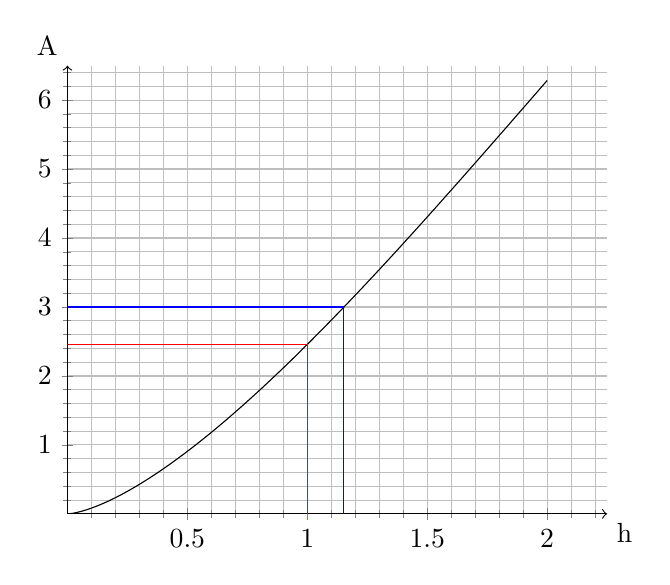
\begin{tikzpicture}
        \begin{axis}[
            axis lines = middle,grid=both,
            axis line style={->},
            minor tick num=4,
            xtick={0,0.5,1,1.5,2,2.5},
            ytick={0,1,2,3,4,5,6,7},
            xmin = 0, xmax=2.25, ymin=0, ymax=6.5,
            x label style={at={(current axis.right of origin)},anchor=north, below right},
            y label style={at={(current axis.above origin)},anchor=south east, above left},
            xlabel={h},
            ylabel={A}
            ]
            \addplot [samples=100, domain=0:2] {2^2 * acos((2-x)/2)*pi/180-(2-x)*sqrt(2^2-(2-x)^2)};
            \draw [red] (axis cs:1,0) |- (axis cs: 0,2.4567);
            \draw [blue] (axis cs:1.15,0) |- (axis cs: 0,3);
        \end{axis}
    \end{tikzpicture}
\end{frame}

\begin{frame}{Método da bissecção}
    \textit{Problema}: Determinar \(x\) tal que \(f(x)=0\)

    \centering
    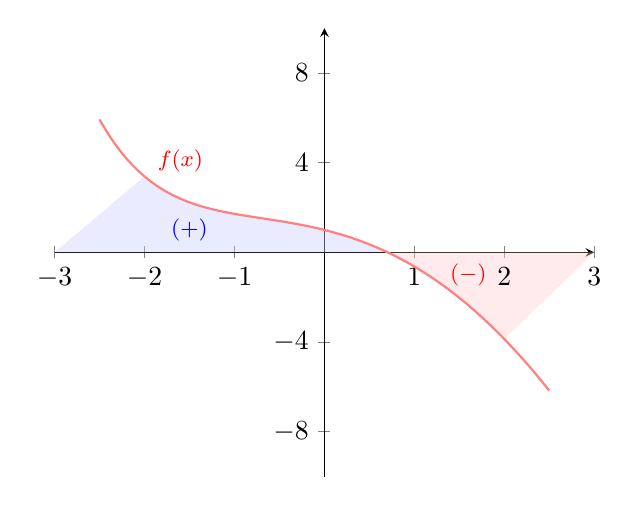
\begin{tikzpicture}

        \begin{axis}[
            xmin=-3, xmax=3,
            ymin=-10, ymax=10,
            xtick distance=1, ytick distance=4,
            axis x line=center,
            axis y line=center
            ]

            \addplot [domain=-2.5:-2, samples=100, thick, color=red!50] {exp(-x)-x^2};
            \addplot [domain=-2:0.567, samples=100, name path=f1, thick, color=red!50] {exp(-x)-x^2};
            \addplot [domain=0.567:2, samples=100, name path=f2, thick, color=red!50] {exp(-x)-x^2};
            \addplot [domain=2:2.5, samples=100, thick, color=red!50] {exp(-x)-x^2};

            \node[color=red, font=\footnotesize] at (-1.6,4.1) {$f(x)$};

            \only<2>{
                \path [name path=g1] (-3,0) -- (0.567,0);
                \path [name path=g2] (0.567,0) -- (3,0);

                \addplot[blue!20, opacity=0.4] fill between [of=f1 and g1];
                \addplot[red!20, opacity=0.4] fill between [of=f2 and g2];

                \node[color=blue, font=\footnotesize] at (-1.5,1) {$(+)$};
                \node[color=red, font=\footnotesize] at (1.6,-1) {$(-)$};
            }
        \end{axis}

    \end{tikzpicture}
\end{frame}

\begin{frame}{Método da bissecção}
    \textit{Problema}: Determinar \(x\) tal que \(f(x)=0\)

    \centering
    \begin{tikzpicture}

        \begin{axis}[
            xmin=-3, xmax=3,
            ymin=-10, ymax=10,
            xtick distance=1, ytick distance=4,
            axis x line=center,
            axis y line=none
            ]

            \addplot [domain=-2.5:-2, samples=100, thick, color=red!50] {exp(-x)-x^2};
            \addplot [domain=-2:0.567, samples=100, name path=f1, thick, color=red!50] {exp(-x)-x^2};
            \addplot [domain=0.567:2, samples=100, name path=f2, thick, color=red!50] {exp(-x)-x^2};
            \addplot [domain=2:2.5, samples=100, thick, color=red!50] {exp(-x)-x^2};

            \node[color=red, font=\footnotesize] at (-1.6,4.1) {$f(x)$};

            \path [name path=g1] (-3,0) -- (0.567,0);
            \path [name path=g2] (0.567,0) -- (3,0);

            \addplot[blue!20, opacity=0.4] fill between [of=f1 and g1];
            \addplot[red!20, opacity=0.4] fill between [of=f2 and g2];

            \node[color=blue, font=\footnotesize] at (-1.5,1) {$(+)$};
            \node[color=red, font=\footnotesize] at (1.6,-1) {$(-)$};

            \only<2-3>{
                \draw[dashed, black!70, below] (0,-6) node (xr) {$x_r$} -- (0,6) ;
                \draw[dashed, black!70, below] (-2,-6) node (xa) {$x_a$} -- (-2,6) ;
                \draw[dashed, black!70, below] (2,-6) node (xb) {$x_b$} -- (2,6) ;
            }

            \only<3> {
                \draw[->, red] (xa.south) to [out=330,in=-150] (xr.south);
            }

            \only<4-5>{
                \draw[dashed, black!70, below] (1,-6) node (xr) {$x_r$} -- (1,6) ;
                \draw[dashed, black!70, below] (0,-6) node (xa) {$x_a$} -- (0,6) ;
                \draw[dashed, black!70, below] (2,-6) node (xb) {$x_b$} -- (2,6) ;
            }

            \only<5> {
                \draw[->, red] (xb.south) to [out=-150,in=-30] (xr.south);
            }

            \only<6-7>{
                \draw[dashed, black!70, below] (0.5,-6) node (xr) {$x_r$} -- (0.5,6) ;
                \draw[dashed, black!70, below] (0,-6) node (xa) {$x_a$} -- (0,6) ;
                \draw[dashed, black!70, below] (1,-6) node (xb) {$x_b$} -- (1,6) ;
            }

            \only<7> {
                \draw[->, red] (xa.south) to [out=-30,in=-150] (xr.south);
            }

        \end{axis}

    \end{tikzpicture}
\end{frame}

\begin{frame}{Método da bissecção}
    \begin{enumerate}
        \item Reescreve-se o problema de forma que se torne ''Determinar \(x\) tal que \(f(x)=0\)''
        \item Estima-se dois valores, $x_a$ e $x_b$ tal que $f(x_a)$ e $f(x_b)$ tenham sinais diferentes
        \item \label{calculo} Calcula-se o ponto médio \(x_r\) do intervalo formado por $x_a$ e $x_b$:
            \[
                x_r=\frac{x_a + x_b}{2}
            \]
        \item \label{escolha} Se o sinal de $f(x_a)$ é igual ao de $f(x_r)$ , então $x_a = x_r$, senão $x_b=x_r$
        \item Repetimos \ref{calculo} e \ref{escolha} até $f(x_r)=0$ ou \textit{outro critério de parada}
    \end{enumerate}

    \pause
    \begin{tcolorbox}[colback=red!10]
        Atividade: Determine \(h\) tal que
        \[
            A=r^2 \arccos{\left(\frac{r-h}{r}\right)}-(r-h)\sqrt{r^2-(r-h)^2}
        \]
        onde \(A=\SI{3}{m^2}\) e \(r=\SI{2}{m}\)
    \end{tcolorbox}
\end{frame}

\begin{frame}{Tabela}
    \(\rightarrow\) A iteração 0 é onde \textit{escolhemos} o ponto de partida do método

    \centering
    \begin{tabular}{c|P{1.75cm}|P{1.75cm}|P{1.75cm}|P{1.75cm}|P{1.75cm}|P{1.75cm}}
        \(i\) & \(h_a\) & \(h_b\) & \(h_r\) & \(f(h_a)\) & \(f(h_b)\) & \(f(h_r)\) \\ \hline\pause
        0 & 0,00000 & 2,00000 & 1,00000 & 3,00000 & -3,28319 & 0,54326 \\ \hline\pause
        1 & 1,00000 & 2,00000 & 1,50000 & 0,54326 & -3,28319 & -1,30422 \\ \hline\pause
        2 & 1,00000 & 1,50000 & 1,25000 & 0,54326 & -1,30422 & -0,35506 \\ \hline\pause
        3 & 1,00000 & 1,25000 & 1,12500 & 0,54326 & -0,35506 & 0,10171 \\ \hline\pause
        4 & 1,12500 & 1,25000 & 1,18750 & 0,10171 & -0,35506 & -0,12494 \\ \hline\pause
        5 & 1,12500 & 1,18750 & 1,15625 & 0,10171 & -0,12494 & -0,01116 \\ \hline\pause
        6 & 1,12500 & 1,15625 & 1,14063 & 0,10171 & -0,01116 & 0,04539 \\ \hline\pause
        7 & 1,14063 & 1,15625 & 1,14844 & 0,04539 & -0,01116 & 0,01715 \\ \hline\pause
        8 & 1,14844 & 1,15625 & 1,15234 & 0,01715 & -0,01116 & 0,00300 \\ \hline\pause
        9 & 1,15234 & 1,15625 & 1,15430 & 0,00300 & -0,01116 & -0,00408 \\ \hline\pause
        10 & 1,15234 & 1,15430 & 1,15332 & 0,00300 & -0,00408 & -0,00054 \\ \hline\pause
        11 & 1,15234 & 1,15332 & 1,15283 & 0,00300 & -0,00054 & 0,00123 \\ \hline\pause
        12 & 1,15283 & 1,15332 & 1,15308 & 0,00123 & -0,00054 & 0,00035
    \end{tabular}
\end{frame}

\begin{frame}{Tabela (continuação)}
    \begin{center}
        \begin{tabular}{c|P{1.75cm}|P{1.75cm}|P{1.75cm}|P{1.75cm}|P{1.75cm}|P{1.75cm}}
            \(i\) & \(x_a\) & \(x_b\) & \(x_r\) & \(f(x_a)\) & \(f(x_b)\) & \(f(x_r)\) \\ \hline
            13 & 1,15308 & 1,15332 & 1,15320 & 0,00035 & -0,00054 & -0,00009 \\ \hline
            14 & 1,15308 & 1,15320 & 1,15314 & 0,00035 & -0,00009 & 0,00013 \\ \hline
            15 & 1,15314 & 1,15320 & 1,15317 & 0,00013 & -0,00009 & 0,00002 \\ \hline
            16 & 1,15317 & 1,15320 & 1,15318 & 0,00002 & -0,00009 & -0,00004 \\ \hline
            17 & 1,15317 & 1,15318 & 1,15318 & 0,00002 & -0,00004 & -0,00001 \\ \hline
            18 & 1,15317 & 1,15318 & 1,15317 & 0,00002 & -0,00001 & 0,00000 \\ \hline
            19 & 1,15317 & 1,15318 & 1,15317 & 0,00000 & -0,00001 & 0,00000 \\ \hline
            20 & 1,15317 & 1,15317 & 1,15317 & 0,00000 & 0,00000 & 0,00000 \\ \hline
            21 & 1,15317 & 1,15317 & 1,15317 & 0,00000 & 0,00000 & 0,00000 \\ \hline
            22 & 1,15317 & 1,15317 & 1,15317 & 0,00000 & 0,00000 & 0,00000 \\ \hline
            23 & 1,15317 & 1,15317 & 1,15317 & 0,00000 & 0,00000 & 0,00000 \\ \hline
            24 & 1,15317 & 1,15317 & 1,15317 & 0,00000 & 0,00000 & 0,00000 \\ \hline
        \end{tabular}
    \end{center}
\end{frame}

\begin{frame}{A função \textit{SE}}
    \begin{itemize}
        \item A função \textit{SE} ''retorna um valor se uma expressão lógica for verdadeira e outro se for falsa'':
            \begin{center}
                \fbox{\texttt{=SE(expressão\_lógica; valor\_se\_verdadeiro; valor\_se\_falso)}}
                \vspace{1em}
            \end{center}
        \item Assumindo que \(x_a\) está B2, \(x_b\) está C2, \(x_r\) está D2, \(f(x_a)\) está em E2, \(f(x_b)\) está em F2 e \(f(x_r)\) está em G2, a expressão
            \begin{center}
                \fbox{\texttt{=SE(E2*G2>=0; D2; B2)}}
                \vspace{1em}
            \end{center}
            será igual a \(x_r\) se \(f(x_a)\) tiver o mesmo sinal que \(f(x_r)\), caso contrário a expressão será igual a \(x_a\)
    \end{itemize}
\end{frame}

\begin{frame}{Exercícios}
    Determine \(x\) (ou \(h\)) tal que
    \begin{enumerate}
        \item \(r^2 \arccos{\left(\frac{r-h}{r}\right)}-(r-h)\sqrt{r^2-(r-h)^2}=3\) onde \(r=2\)
        \item \(e^{-x}=x\)
        \item \(\ln(x-1) + \cos(x-1)=0 \)
        \item \(e^x=3x^2\)
        \item \((x-2)^2=\ln x\)
    \end{enumerate}
\end{frame}

\begin{frame}
    \frametitle{Método de Newton-Raphson}

    Sendo \(x_0\) uma aproximação inicial (''chute''), podemos obter uma aproximação ''melhor'' através da fórmula
    \begin{block}
        {}
        \[ x_{k+1} = x_k - \frac{f(x_k)}{f'(x_k)} \]
    \end{block}
    onde \(k=0,1,2,\ldots\) é o número da \textbf{iteração}. 

    O método de Newton-Raphson
    \begin{itemize}
        \item É um método \textit{aberto}, isto é, é necessário apenas um valor inicial \(x_0\)
        \item Algumas vezes \textit{diverge}, ou seja, o resultado obtido em cada iteração se afasta da raiz verdadeira
        \item Mas quando há convergência o resultado obtido em cada iteração se aproxima da raiz verdadeira muito mais rápido do que o método da bissecção
    \end{itemize}
\end{frame}

\begin{frame}{Atividade}
    \begin{itemize}
        \item Determine \(x\) tal que \(f(x)=0\) onde
            \[
                \color{blue}
                \boxed{f(x)=x^2+3x-4}
            \]
            usando o método de Newton Raphson com derivada analítica
            \[
                \color{blue}
                \boxed{f'(x)=2x+3}
            \]
    \end{itemize}
\end{frame}

\begin{frame}{Atividade}
    Determine \(h\) tal que

    \[
        \color{blue}
        r^2 \arccos{\left(\frac{r-h}{r}\right)}-(r-h)\sqrt{r^2-(r-h)^2}=3
    \]
    onde \(r=2\) usando o método de Newton Raphson com derivada analítica
    \[
        \color{blue}
        \frac{d}{dx} \left( 
            r^2 \arccos{\left(\frac{r-h}{r}\right)}-(r-h)\sqrt{r^2-(r-h)^2}
        \right)=
        2\sqrt{h(2r-h)}
    \]
\end{frame}

\begin{frame}
\end{frame}
\begin{frame}
    \frametitle{Sistemas de equações lineares}
    Um sistema de equações lineares consiste em um conjunto de $m$ equações lineares com $n$ variáveis de $x_i$:

    \begin{align*}
        a_{11} x_1 + a_{12} x_2 + a_{13} x_3 + \cdots  + a_{1n} x_n & =  b_1 \\
        a_{21} x_1 + a_{22} x_2 + a_{23} x_3 + \cdots + a_{2n} x_n & =  b_2 \\
        a_{31} x_1 + a_{32} x_2 + a_{33} x_3 + \cdots + a_{3n} x_n & = b_3 \\
                                                                   & ~\vdots~ \\
        a_{m1} x_1 + a_{m2} x_2 + a_{m3} x_3 + \cdots  + a_{mn} x_n & =  b_m
    \end{align*}
\end{frame}

\begin{frame}
    \frametitle{Sistema de equações lineares - forma matricial}
    O sistema anterior pode ser representado na forma matricial por:

    \[
        \begin{bmatrix}
            a_{11} & a_{12} & a_{13} & \cdots & a_{1n}  \\
            a_{21} & a_{22} & a_{23} & \cdots & a_{2n}  \\
            a_{31} & a_{32} & a_{33} & \cdots & a_{3n}  \\
                   &        &        & \vdots &         \\
            a_{m1} & a_{m2} & a_{m3} & \cdots & a_{mn}
        \end{bmatrix}
        \begin{bmatrix}
            x_1 \\ x_2 \\ x_3 \\ \vdots \\ x_n
        \end{bmatrix}=
        \begin{bmatrix}
            b_1 \\ b_2 \\ b_3 \\ \vdots \\ b_m
        \end{bmatrix}
    \]

    ou simplesmente $Ax=b$, onde $A$ é chamada de matriz de coeficientes, $x$ é o vetor solução e $b$ é o vetor dos termos independentes. Resolver um sistema consiste em encontrar um vetor $x$ que satisfaça simultaneamente às equações.

    \pause 

    Se $A$ for uma matriz quadrada ($m = n$) não singular ($det(A) \neq 0$), então:

    \[
        Ax=b ~\rightarrow~ A^{-1}Ax=A^{-1}b ~\rightarrow~ x=A^{-1}b
    \]
\end{frame}

\begin{frame}
    \frametitle{Sistema triangular superior}

    Seja um sistema triangular superior 3x3
    \[
        \begin{bmatrix}
            a_{11} & a_{12} & a_{13} \\
            0      & a_{22} & a_{23} \\
            0      & 0      & a_{33}
        \end{bmatrix}
        \begin{bmatrix}
            x_1 \\ x_2 \\ x_3
        \end{bmatrix}
        =
        \begin{bmatrix}
            b_1 \\ b_2 \\ b_3
        \end{bmatrix}
    \]

    O vetor solução \( x\) pode ser obtido através de substituições retroativas:
    \begin{align*}
        x_3 &= \frac{b_3}{a_{33}} \\
        x_2 & = \frac{b_2 - a_{23}x_3}{a_{22}} \\
        x_1 &= \frac{b_1 - a_{12}x_2 - a_{13}x_3}{a_{11}}
    \end{align*}
\end{frame}

\begin{frame}
    Ou seja,

    \[
        x_i = \frac{b_i - \sum_{j=i+1}^{3} {a_{ij} x_j}}{a_{ii}}
    \]
    onde \(i = 3, 2, 1\). Para um sistema \(n\) x \(n\), temos
    \[
        x_i = \frac{b_i - \sum_{j=i+1}^{n} {a_{ij} x_j}}{a_{ii}}
    \]
    onde \(i = n, n-1, n-2, \ldots , 1\)

    \begin{block}{Eliminação de Gauss}
        O método de eliminação de Gauss consiste em transformar um sistema de equações lineares em um sistema triangular superior equivalente e obter o vetor solução através de substituições retroativas
    \end{block}
\end{frame}

\begin{frame}
    Um sistema linear pode ser transformado em outro equivalente através das operações
    \begin{itemize}
        \item Trocar a ordem de duas equações
        \item Multiplicar uma equação por uma constante não nula
        \item Somar duas equações
    \end{itemize}

    \begin{block}
        {Exemplo}
        Resolva o seguinte sistema usando eliminação de Gauss

        \[
            \begin{bmatrix}
                10 & 3 & -2 \\ 2 & 8 & -1 \\ 1 & 1 & 5
            \end{bmatrix}
            \begin{bmatrix}
                x_1 \\ x_2 \\ x_3
            \end{bmatrix}
            =
            \begin{bmatrix}
                57 \\ 20 \\ -4
            \end{bmatrix}
        \]

    \end{block}
\end{frame}

\begin{frame}
    \frametitle{Primeira etapa}
    Como as operações envolvem as equações, tanto \(A\) quanto \(b\) são modificadas. Assim, é interessante construir uma matriz ''aumentada'' \([A,b]\):

    \[
        [A,b] =
        \left[
            \begin{array}{ccc|c}
                10 & 3 & -2 & 57 \\ 2 & 8 & -1 & 20 \\ 1 & 1 & 5 & -4
            \end{array}
        \right]
    \]

    de maneira que as operações ocorrendo em \(A\) também ocorram em \(b\). 

    \begin{block}
        {}
        Em uma matriz triangular superior, todos os elementos abaixo da diagonal são nulos. Assim, devemos zerar todos os elementos abaixo da diagonal
    \end{block}

\end{frame}

\begin{frame}
    \frametitle{Segunda etapa}

    \begin{enumerate}
        \item ''Somamos'' a segunda equação (\(L_2\)) com a primeira (\(L_1\)) multiplicada por uma constante, de forma que o elemento \(a_{21} = 0\)
            \[
                L_2 \leftarrow L_2 - \frac{a_{21}}{a_{11}} L_1
            \] 
        \item ''Somamos'' a terceira equação (\(L_3\)) com a primeira (\(L_1\)) multiplicada por uma constante, de forma que o elemento \(a_{31} = 0\)
            \[
                L_3 \leftarrow L_3 - \frac{a_{31}}{a_{11}} L_1
            \] 
    \end{enumerate}
    \[
        \left[
            \begin{array}{ccc|c}
                10 & 3 & -2 & 57 \\ 2 & 8 & -1 & 20 \\ 1 & 1 & 5 & -4
            \end{array}
        \right]
        \rightarrow
        \left[
            \begin{array}{ccc|c}
                10 & 3 & -2 & 57 \\ 0 & 37/5 & -3/5 & 43/5 \\ 0 & 7/10 & 26/5 & -97/10
            \end{array}
        \right]
    \]
\end{frame}

\begin{frame}
    \frametitle{Terceira etapa}
    \begin{enumerate}
        \item ''Somamos'' a terceira equação (\(L_3\)) com a segunda (\(L_2\)) multiplicada por uma constante, de forma que o elemento \(a_{32} = 0\)
            \[
                L_3 \leftarrow L_3 - \frac{a_{32}}{a_{22}} L_2
            \] 
    \end{enumerate}
    \[
        \left[
            \begin{array}{ccc|c}
                10 & 3 & -2 & 57 \\ 0 & 37/5 & -3/5 & 43/5 \\ 0 & 7/10 & 26/5 & -97/10
            \end{array}
        \right]
        \rightarrow
        \left[
            \begin{array}{ccc|c}
                10 & 3 & -2 & 57 \\ 0 & 37/5 & -3/5 & 43/5 \\ 0 & 0 & 389/74 & -389/37
            \end{array}
        \right]
    \]
\end{frame}

\begin{frame}
    \frametitle{Quarta etapa}
    Resolvemos o sistema triangular superior usando a expressão
    \[
        x_i = \frac{b_i - \sum_{j=i+1}^{n} {a_{ij} x_j}}{a_{ii}}
    \]
    onde \(i = n, n-1, n-2, \ldots , 1\)

    \begin{align*}
        x_3 &= \frac{-389/37}{389/74}=-2 \\
        x_2 & =\frac{43/5 - (-3/5)*(-2)}{37/5}=1 \\
        x_1 &= \frac{57-3*1-(-2)*(-2)}{10} = 5
    \end{align*}

\end{frame}


\begin{frame}{Sistema de equações lineares - planilha eletrônica}
    \begin{itemize}
        \item Seja o sistema na forma matricial \(Ax=b\):
            \[
                \begin{bmatrix}
                    a_{11} & a_{12} & a_{13} & \cdots & a_{1n}  \\
                    a_{21} & a_{22} & a_{23} & \cdots & a_{2n}  \\
                    a_{31} & a_{32} & a_{33} & \cdots & a_{3n}  \\
                           &        &        & \vdots &         \\
                    a_{m1} & a_{m2} & a_{m3} & \cdots & a_{mn}
                \end{bmatrix}
                \begin{bmatrix}
                    x_1 \\ x_2 \\ x_3 \\ \vdots \\ x_n
                \end{bmatrix}=
                \begin{bmatrix}
                    b_1 \\ b_2 \\ b_3 \\ \vdots \\ b_m
                \end{bmatrix}
            \]
        \item Como vimos, podemos resolvê-lo encontrando a matriz inversa de \(A\)
            \[
                Ax=b \implies x=A^{-1}b
            \]
        \item Para matrizes pequenas, podemos usar as funções \texttt{MATRIZ.MULT} e \texttt{MATRIZ.INVERSO}
    \end{itemize}
\end{frame}

\begin{frame}[c]{Planilha eletrônica}

\begin{itemize}
    \item Temos que \(Ax=b ~\rightarrow~ A^{-1}Ax=A^{-1}b ~\rightarrow~ x=A^{-1}b\)
    \item A função \texttt{MATRIZ.MULT(matriz1; matriz2)} multiplica duas matrizes
    \item A função \texttt{MATRIZ.INVERSO(matriz\_quadrada)} calcula a inversa de uma matriz quadrada
    \item Se colocarmos a matriz \(A\) nas células \texttt{A1:G7} e a matriz \(b\) em \texttt{H1:H7}, a matriz \(x\) pode ser calculada por
    \begin{center}
        \texttt{=MATRIZ.MULT(MATRIZ.INVERSO(A1:G7);H1:H7)}
    \end{center}
\end{itemize}
    
\end{frame}

\begin{frame}[c]{Mas nem tudo são flores...}
 Essas funções têm particularidades dependendo da planilha
 \begin{itemize}
        \item \textbf{LibreOffice}: para finalizar a entrada do comando você deve digitar \texttt{Ctrl-Shift-Enter} ao invés de apenas \texttt{Enter}
        \item \textbf{Excel}: antes de entrar o comando você deve selecionar o número de células que serão ocupadas e para finalizar a entrada do comando você deve digitar \texttt{Ctrl-Shift-Enter} ao invés de apenas \texttt{Enter}
        \item \textbf{Google Planilhas}: para finalizar a entrada do comando você deve digitar \texttt{Ctrl-Shift-Enter} seguido de \texttt{Enter} ao invés de apenas \texttt{Enter}
    \end{itemize}

\end{frame}

\begin{frame}{Exercícios extras}
Encontre as soluções dos sistemas lineares abaixo usando uma planilha eletrônica:

\begin{columns}
    \begin{column}{0.45\textwidth}
        \begin{enumerate}
            \item \systeme*{-4x+2y=5,-x-9y+5z=6,x-3y+4z=9} 
            \item \systeme*{6x-y-8z=-5,-6x+4y-2z=7,4x+9y-8z=-7}
            \item \systeme*{x-5y+9z=5,y-z=-8,8x-3y+6z=-3}
        \end{enumerate}
    \end{column}
    
    \begin{column}{0.45\textwidth}
        \begin{enumerate}\addtocounter{enumi}{3}
            \item \systeme*{-t-5u+8v+6w=-3,3t+u+4v-w=6,-6t-u+8v-5w=6,-7t+3u-3v=3}
            \item \systeme*{2t+9u+8v+4w=4,-9t-8u-9v+9w=-5,-7t-7u+2v+4w=-5,3t+6u=4}
        \end{enumerate}    
    \end{column}
\end{columns}

\end{frame}

\begin{frame}
\frametitle{Sistemas não lineares}

O sistema a seguir é formado por um conjunto de duas equações simultâneas não lineares com duas incógnitas
\[
\begin{cases}
x_1^2 + x_1x_2 &= 10 \\
x_2 + 3x_1x_2^2 &= 57
\end{cases}
\]

Podemos expressar esse sistema na forma

\[
\begin{cases}
x_1^2 + x_1x_2 -10 &= 0 \\
x_2 + 3x_1x_2^2 -57 &= 0
\end{cases}
\]

ou seja: a solução do sistema são os os valores de $x_1$ e $x_2$ que tornam as equações iguais a zero
\end{frame}

\begin{frame}[c]
De forma geral, qualquer sistema não linear pode ser expresso na forma
\[
\begin{cases}
f_1(x_1, x_2, \ldots, x_n) =& 0 \\
f_2(x_1, x_2, \ldots, x_n) =& 0 \\
                         \vdots & \\
f_n(x_1, x_2, \ldots, x_n) =& 0 \\                           
\end{cases}
\]

e para encontrar a solução basta encontrar os zeros das funções. O problema reside no fato de $f_1$, $f_2$, $\ldots$, $f_n$ serem funções de mais de uma variável
\end{frame}

\begin{frame}
\frametitle{Método de Newton-Raphson}
Devemos definir um vetor solução inicial $x^0$ e encontrar o vetor solução $x^{k+1}$ através da fórmula
\[
\color{blue} 
x^{k+1}=x^k-J^{-1} f
\]
onde

\[
\color{red}
J=
\begin{bmatrix}
\left. \dfrac{\partial f_1}{\partial x_1}\right|_{x_1^k,x_2^k,\ldots,x^k_N} &
\left. \dfrac{\partial f_1}{\partial x_2}\right|_{x_1^k,x_2^k,\ldots,x^k_N} & \ldots &
\left. \dfrac{\partial f_1}{\partial x_N}\right|_{x_1^k,x_2^k,\ldots,x^k_N} \\
\left. \dfrac{\partial f_2}{\partial x_1}\right|_{x_1^k,x_2^k,\ldots,x^k_N} &
\left. \dfrac{\partial f_2}{\partial x_2}\right|_{x_1^k,x_2^k,\ldots,x^k_N} & \ldots &
\left. \dfrac{\partial f_2}{\partial x_N}\right|_{x_1^k,x_2^k,\ldots,x^k_N} \\
\vdots & \vdots & \ddots & \vdots \\
\left. \dfrac{\partial f_N}{\partial x_1}\right|_{x_1^k,x_2^k,\ldots,x^k_N} &
\left. \dfrac{\partial f_N}{\partial x_2}\right|_{x_1^k,x_2^k,\ldots,x^k_N} & \ldots &
\left. \dfrac{\partial f_N}{\partial x_N}\right|_{x_1^k,x_2^k,\ldots,x^k_N}
\end{bmatrix}
\color{black}
\text{ e }
\color{magenta}
f=
\begin{bmatrix}
f_1(x_1^k,x_2^k,\ldots,x^k_N) \\
f_2(x_1^k,x_2^k,\ldots,x^k_N) \\ \vdots \\
f_N(x_1^k,x_2^k,\ldots,x^k_N)
\end{bmatrix}
\]

\end{frame}

\begin{frame}
\frametitle{Exemplo}
O sistema
\[
\begin{cases}
x_1^2 + x_1x_2 &= 10 \\
x_2 + 3x_1x_2^2 &= 57
\end{cases}
\]
tem

\begin{columns}[T]
\begin{column}{0.45\textwidth}
\[
J=
\begin{bmatrix}
2x_1 + x_2 & x_1 \\
3x_2^2 & 1 + 6x_1x_2 
\end{bmatrix}
\]
\end{column}

\begin{column}{0.45\textwidth}

\[
f=
\begin{bmatrix}
x_1^2 + x_1x_2 - 10 \\
x_2 + 3x_1x_2^2 - 57
\end{bmatrix}
\]
\end{column}
\end{columns}

Usando 
\[
x^0=
\begin{bmatrix}
1,5 \\ 3,5
\end{bmatrix}
\]
temos

\begin{columns}
\begin{column}{0.45\textwidth}
\[
J=
\begin{bmatrix}
6,5 & 1,5 \\
36,75 & 32,5 
\end{bmatrix}
\]
\end{column}

\begin{column}{0.45\textwidth}
\[
f=
\begin{bmatrix}
-2,5 \\
1,625
\end{bmatrix}
\]
\end{column}
\end{columns}
\end{frame}

\begin{frame}[c]
Usando \texttt{MATRIZ.INVERSO}, temos que
\[
J^{-1}=
\begin{bmatrix}
0,2082 &	-0,0096 \\
-0,2354	& 0,0416  \\
\end{bmatrix}
\]

e
\[
\begin{bmatrix}
x_1^1 \\ x_2^1
\end{bmatrix}
=
\begin{bmatrix}
1,5 \\ 3,5
\end{bmatrix}
-
\begin{bmatrix}
0,2082 &	-0,0096 \\
-0,2354	& 0,0416  \\
\end{bmatrix}
\begin{bmatrix}
-2,5 \\
1,625
\end{bmatrix}
=
\begin{bmatrix}
2,0360 \\
2,8439
\end{bmatrix}
\]
\end{frame}

\begin{frame}{Exemplo}
Resolva o seguinte sistema não linear 
\[
\begin{cases}
x_1^2+x_2^2+x_3^2=1 \\
2x_1^2+x_2^2-4x_3=0 \\
3x_1^2-4x_2+x_3=0
\end{cases}
\]
com
\(
x^0=
\begin{bmatrix}
0,5 \\ 0,5 \\ 0,5
\end{bmatrix}
\)
e
\(
J=
\begin{bmatrix}
2x_1 & 2x_2 & 2x_3 \\
4x_1 & 2x_2 & -4 \\
6x_1 & -4 & 1
\end{bmatrix}
\)
\end{frame}



\end{document}
